\documentclass{article}
% PKGS START
\usepackage[utf8x]{inputenc}
\usepackage[english,russian]{babel}
\usepackage{cmap}
\usepackage{commath}
\usepackage{amsmath}
\usepackage{amsfonts}
\usepackage{mathtools}
\usepackage{amssymb}
\usepackage{parskip}
\usepackage{titling}
\usepackage{color}
\usepackage{hyperref}
\usepackage{cancel}
\usepackage{enumerate}
\usepackage{multicol}
\usepackage{graphicx}
\usepackage[font=small,labelfont=bf]{caption}
\usepackage[a4paper, left=2.5cm, right=1.5cm, top=2.5cm, bottom=2.5cm]{geometry}
% PKGS END
% INIT START
\graphicspath{ {./images/} }
\setlength{\droptitle}{-3cm}
\hypersetup{
    colorlinks=true, %set true if you want colored links
    linktoc=all,     %set to all if you want both sections and subsections linked
    linkcolor=blue,  %choose some color if you want links to stand out
}

\pagenumbering{arabic}
% INIT END
\begin{document}
    \section{Непрерывность функции в точке}
    

    \textbf{Определение.} Функция \(y = f(x)\) называется непрерывной в \(x = a\), если 

    \begin{enumerate}
        \item \(f(x)\) определена в \(U(a)\)
        \item \(lim_{x \rightarrow a} f(x) = f(a)\)
        
        Подробнее:

        \( \forall\ \varepsilon > 0\ \exists\ \delta(\varepsilon):\ \forall\ x:\ \abs{x - a} < \delta \Rightarrow \abs{f(x) - f(a)} < \varepsilon \)
        % График с функцией и a-delta; a; a+delta

        \(\exists\ \varepsilon:\ \forall \delta\ \exists\ x:\ \abs{x-a}<\delta\ \abs{f(x)-f(a)} \geq \varepsilon\)
    \end{enumerate}

    \begin{minipage}{0.49\linewidth}
        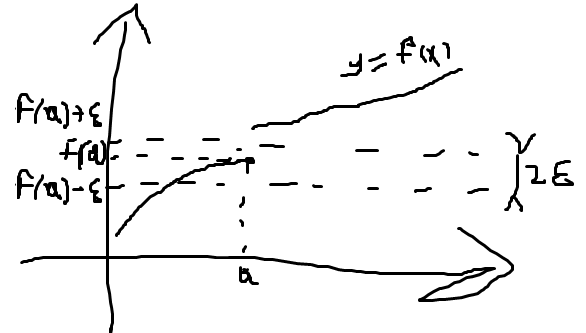
\includegraphics[width=\linewidth]{example_11_1_3_1.png}
        \captionof{figure}{Пример разрывности}
    \end{minipage}
    % Пример разрывности example_11_1_3_1.png

    \subsection{Классификация точек разрыва}
    \(lim_{x \rightarrow a + 0} f(x) = A\)\\
    \(lim_{x \rightarrow a - 0} f(x) = A\)
    
    \textbf{Определение.} Функция \(y = f(x)\) называется непрерывной слева в \(x = a\), если

    \begin{enumerate}
        \item \(f(x)\) определена \( \forall\ x \in (a - \delta; a] \)
        \item \(lim_{x\rightarrow a-0} f(x)=f(a)\)
    \end{enumerate}

    \textbf{Определение.} Функция \(y = f(x)\) называется непрерывной справа в \(x = a\), если
    
    \begin{enumerate}
        \item \(f(x)\) определена \( \forall\ x \in [a; a + \delta) \)
        \item \(lim_{x\rightarrow a+0} f(x)=f(a)\)
    \end{enumerate}

    Понятно, что \( lim_{x \rightarrow a} f(x) = f(a) \Leftrightarrow lim_{x \rightarrow a + 0} f(x) = f(a) = lim_{x \rightarrow a - 0} f(x) \)

    \textbf{Определение.} Если существуют конечные пределы \(lim_{x \rightarrow a+0} f(x)\) и \(lim_{x \rightarrow a-0} f(x)\), но функция разрывна, то в \(x=a\) разрыв 1-го рода.

    \(\begin{cases}{l}\frac{x^2-4}{x-2}\\ 4;\ x=2\end{cases}\)

    \textbf{Определение.} Если в \(x=a\) функция разрывна, и этот разрыв не является разрывом первого рода, то жто разрыв 2-го рода.

    \(y = sin \frac{1}{x}\) в \(x=0\)

    \(x_n'=\frac{2}{\pi+4\pi n} \rightarrow 0\)

    
\end{document}
